\documentclass{beamer}
\usepackage[utf8]{inputenc}
\usepackage{utopia}

\usepackage{amsfonts}
\usepackage{amsmath}		
\usepackage{amssymb}
\usepackage{beamerthemesplit}
\usepackage{bezier}
\usepackage{float}
\usepackage{hyperref}
\usepackage{longtable}
\usepackage{makeidx}
\usepackage{rotating}
\usepackage{wrapfig}
\usepackage{multirow}
\usepackage{pgf}
\usepackage{ragged2e}

\usetheme{Madrid}
\usecolortheme{default}

\title[Graph Neural Networks]{Graph Neural Networks \\ Efficient Tensor Operations In CUDA/GPU \\ Custom Deep Learning Framework In C++ \\ Applications In Quantum Chemistry}
\author[Hy et al.]{Hy Truong Son, Chris Jones \\ Advisor: Prof. Risi Kondor}
\institute[UChicago]{The University of Chicago}
\date{December 2017}

\begin{document}

\logo{
\includegraphics[height=0.5cm]{Logo.jpg}}

\frame{\titlepage}

\begin{frame}
\frametitle{Table of Contents}
\tableofcontents
\end{frame}

\section{Chapter I: Introduction}

\begin{frame}
\frametitle{Our publication}
Covariant Compositional Networks For Learning Graphs (ICLR 2018)
\end{frame}

\begin{frame}
\frametitle{What are Graph Neural Networks?}
\end{frame}

\begin{frame}
\frametitle{What are Tensor Operations?}
\end{frame}

\begin{frame}
\frametitle{What is a Deep Learning framework?}
\end{frame}

\begin{frame}
\frametitle{Molecular Chemical Representation}
\begin{justify}
\begin{center}
	Harvard Clean Energy Project (HCEP) Dataset \cite{Johannes}
\end{center}
\begin{center}
	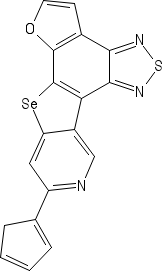
\includegraphics[scale=0.5]{sketcher}
\end{center}
Compound: C18H9N3OSSe \\
SMILES: C1C=CC=C1c1cc2[Se]c3c4occc4c4nsnc4c3c2cn1 \\
Power Conversion Efficiency (PCE, range 0 - 11): 5.16195
\end{justify}
\end{frame}

\begin{frame}
\frametitle{Molecular Graph Representation}
\begin{justify}
\begin{center}
	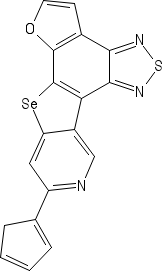
\includegraphics[scale=0.5]{sketcher}
	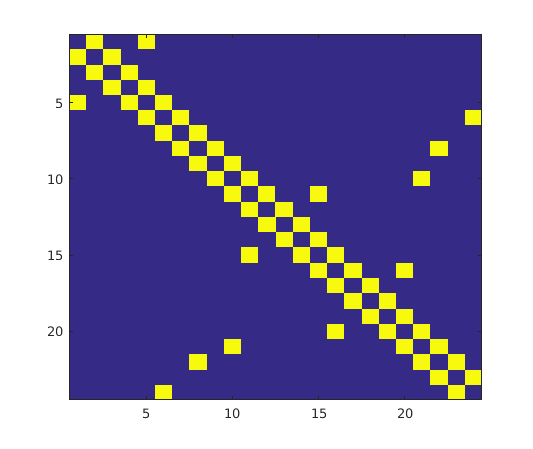
\includegraphics[scale=0.5]{adjacency}
\end{center}
C18H9N3OSSe \ \ \ \ \ \ \ \ \ \ \ \ \ \ \ \ \ \ \ \ Adjacency matrix
\end{justify}
\end{frame}

\section{Chapter II: State-of-the-art Algorithms}

\begin{frame}
\frametitle{Covariant Neural Networks}
\end{frame}

\begin{frame}
\frametitle{Tensor Contractions}
\end{frame}

\begin{frame}
\frametitle{Virtual Indexing System}
\end{frame}

\begin{frame}
\frametitle{GPU Multi-threading}
\end{frame}

\begin{frame}
\frametitle{CPU Multi-threading}
\end{frame}

\section{Chapter III: Experiments and Results}

\begin{frame}
\frametitle{Performance Test: GPU Matrix Multiplication}
\end{frame}

\begin{frame}
\frametitle{Performance Test: GPU Tensor Contractions}
\end{frame}

\begin{frame}
\frametitle{Synthetic Graph Dataset}
\end{frame}

\begin{frame}
\frametitle{Small-scale Molecular Test}
\end{frame}

\begin{frame}
\frametitle{Real-world Dataset}
\end{frame}

\section{Chapter IV: Conclusion and Future Research}

\begin{frame}
\frametitle{Conclusion and Future Research}
\begin{justify}
We implemented the state-of-the-art generalized convolution operation for Graph Neural Networks in order to approximate Density Functional Theory. We obtained very promising results on the Harvard Clean Energy Project dataset.
$$$$
We are developing our custom Deep Learning framework in CUDA/C++ named \textbf{GraphFlow} which supports symbolic differentitation and dynamic computation graph. We expect that this framework will enable us to design more flexible, efficient Graph Neural Networks at a large scale in the future.
\end{justify}
\end{frame}

\begin{frame}
\frametitle{Acknowledgements}
\begin{justify}
We would like to acknowledge my advisor Professor Risi Kondor for his valuable instructions and especially for his great ideas in generalizing convolution operations in graphs. We also want to thank other members of Machine Learning group at the University of Chicago for their dedicated support.
$$$$
Some of the neural network training in this paper was done using the Midway cluster at the UChicago Computing Research Center.
\end{justify}
\end{frame}

\begin{frame}
\frametitle{Reference}
\begin{justify}
\begin{thebibliography}{9}

\bibitem[1]{Nino}
   N. Shervashidze, P. Schweitzer, E. J. van Leeuwen, K. Mehlhorn, K. M. Borgwardt,
   ``Weisfeiler-Lehman Graph Kernels'',
   \textit{Journal of Machine Learning Research}, vol.~12, 2011.
   
\bibitem[2]{Johannes}
   J. Hachmann, R. O. Amaya, S. A. Evrenk, C. A. Bedolla, R. S. S. Carrera, A. G. Parker, L. Vogt, A. M. Brockway, and A. A. Guzik,
   ``The Harvard Clean Energy Project: Large-Scale Computational Screening and Design of Organic Photovoltaics on the World Community Grid'',
   \textit{The Journal of Physical Chemistry Letters}, pp.~2241--2251, 2011.

\bibitem[3]{Risi}
   R. I. Kondor, and J. Lafferty,
   ``Diffusion Kernels on Graphs and Other Discrete Structures'',
   \textit{International Conference on Machine Learning (ICML)}, 2002.
   
\end{thebibliography}
\end{justify}
\end{frame}

\begin{frame}
\frametitle{Reference}
\begin{justify}
\begin{thebibliography}{9}

\bibitem[4]{Nils}
   N. M. Kriege, P. L. Giscard, R. C. Wilson,
   ``On Valid Optimal Assignment Kernels and Applications to Graph Classification'',
   \textit{Neural Information Processing Systems (NIPS)}, 2016.

\bibitem[5]{Steven}
   S. Kearnes, K. McCloskey, M. Berndl, V. Pande, P. Riley,
   ``Molecular Graph Convolutions: Moving Beyond Fingerprints'',
   \textit{Journal of Computer-Aided Molecular Design}, vol.~30, pp.~595--608, 2016.

\bibitem[6]{Duvenaud}
   D. Duvenaud, D. Maclaurin, J. A. Iparraguirre, R. G. Bombarelli, T. Hirzel, A. A. Guzik, R. P. Adams,
   ``Convolutional Networks on Graphs for Learning Molecular Fingerprints'',
   \textit{Neural Information Processing Systems (NIPS)}, 2015.
  
\end{thebibliography}
\end{justify}
\end{frame}

\begin{frame}
\frametitle{Reference}
\begin{justify}
\begin{thebibliography}{9}
   
\bibitem[7]{Thomas}
   T. N. Kipf, M. Welling,
   ``Semi-Supervised Classification with Graph Convolutional Networks'',
   \textit{International Conference on Learning Representations (ICLR)}, 2017.

\bibitem[8]{Maaten}
   L. V. D. Maaten, G. Hinton,
   ``Visualizing Data using t-SNE'',
   \textit{Journal of Machine Learning Research}, vol.~9, pp.~2579--2605, 2008.

\end{thebibliography}
\end{justify}
\end{frame}

\begin{frame}
\frametitle{}
\begin{center}
Thank you very much for your attention!
\end{center}
\end{frame}


\end{document}